\documentclass{beamer}
\usepackage[orientation=landscape,size=a0,scale=1.2]{beamerposter}
\usepackage{haziq_poster_landscape}
\usepackage{haziq_maths}

%%%%%%%%%%%%%%%%%%%%%%%%%%%%%%%%%%%%%%%%%%%%%%%%%%%%%%%%%%%%%%%%%%%%%%%%%%%%%%%%
%%% POSTER SETTINGS %%%%%%%%%%%%%%%%%%%%%%%%%%%%%%%%%%%%%%%%%%%%%%%%%%%%%%%%%%%%
%%%%%%%%%%%%%%%%%%%%%%%%%%%%%%%%%%%%%%%%%%%%%%%%%%%%%%%%%%%%%%%%%%%%%%%%%%%%%%%%
\setbeamercolor{block title}{fg=black,bg=white}
\setbeamercolor{block body}{fg=black,bg=white}
\setbeamercolor{block alerted title}{fg=white,bg=black}
\setbeamercolor{block alerted body}{fg=black,bg=white}

% Define the column widths and overall poster size
% To set effective sepwid, onecolwid and twocolwid values, first choose how many columns you want and how much separation you want between columns
% In this template, the separation width chosen is 0.024 of the paper width and a 4-column layout
% onecolwid should therefore be (1 - sepwid * (# of columns + 1)) / # of columns 
% e.g. (1 - 0.024 * (4 + 1)) / 4 = 0.22
% Set twocolwid to be (2 * onecolwid) + sepwid = 0.464
% Set threecolwid to be (3 * onecolwid) + 2 * sepwid = 0.708
% The whole poster consists of three major columns, the second of which is split into two columns twice - the [t] option aligns each column's content to the top
% A0 is 841 x 1189 mm
% A1 is 594 x 841 mm
% sep      =  28.536 mm
% half sep =  14.268 mm
% onecol   = 261.580 mm
% total    = 304.384 mm
\newlength{\sepwid}
\newlength{\onecolwid}
\newlength{\twocolwid}
\newlength{\threecolwid}
\setlength{\sepwid}{0.024\paperwidth} % Separation width (white space) between columns
\setlength{\onecolwid}{0.22\paperwidth} % Width of one column
\setlength{\twocolwid}{0.464\paperwidth} % Width of two columns
\setlength{\threecolwid}{0.708\paperwidth} % Width of three columns

% Title section
\title{
  Binary and Multinomial Regression using Fisher\\[0.4ex] 
  Information Covariance Kernels (I-priors)
}

\author{Haziq J \& W Bergsma}

\institute{
  Department of Statistics\\
  London School of Economics and\\[0.3ex] 
  Political Science\\[0.7ex]
  \url{https://phd.haziqj.ml}
}

%%%%%%%%%%%%%%%%%%%%%%%%%%%%%%%%%%%%%%%%%%%%%%%%%%%%%%%%%%%%%%%%%%%%%%%%%%%%%%%%
%%% BEGIN DOCUMENT %%%%%%%%%%%%%%%%%%%%%%%%%%%%%%%%%%%%%%%%%%%%%%%%%%%%%%%%%%%%%
%%%%%%%%%%%%%%%%%%%%%%%%%%%%%%%%%%%%%%%%%%%%%%%%%%%%%%%%%%%%%%%%%%%%%%%%%%%%%%%%
\begin{document}
\begin{frame}[t]  % the whole poster is enclosed in one beamer frame
\vspace{-0.3cm}
\begin{columns}[t]  % and in the columns environment

% Draw lines separating columns
\tikz[remember picture,overlay]{\draw[black,thick] ([shift={(305mm,-11.5cm)}]current page.north west) -- ([shift={(305mm,1.6cm)}]current page.south west);} % Left
\tikz[remember picture,overlay]{\draw[black,thick] ([shift={(0mm,-32.9cm)}]current page.north) -- ([shift={(0mm,24cm)}]current page.south);}
\tikz[remember picture,overlay]{\draw[black,thick] ([shift={(-305mm,-11.5cm)}]current page.north east) -- ([shift={(-305mm,24cm)}]current page.south east);}

%%%%%%%%%%%%%%%%%%%%%%%%%%%%%%%%%%%%%%%%%%%%%%%%%%%%%%%%%%%%%%%%%%%%%%%%%%%%%%%%
%%% FIRST COLUMN %%%%%%%%%%%%%%%%%%%%%%%%%%%%%%%%%%%%%%%%%%%%%%%%%%%%%%%%%%%%%%%
%%%%%%%%%%%%%%%%%%%%%%%%%%%%%%%%%%%%%%%%%%%%%%%%%%%%%%%%%%%%%%%%%%%%%%%%%%%%%%%%
\spacercolumn\hspace{-7mm}
\begin{column}{\onecolwid} % The first column

\vspace{-0.8cm}
\begin{figure}[t]
  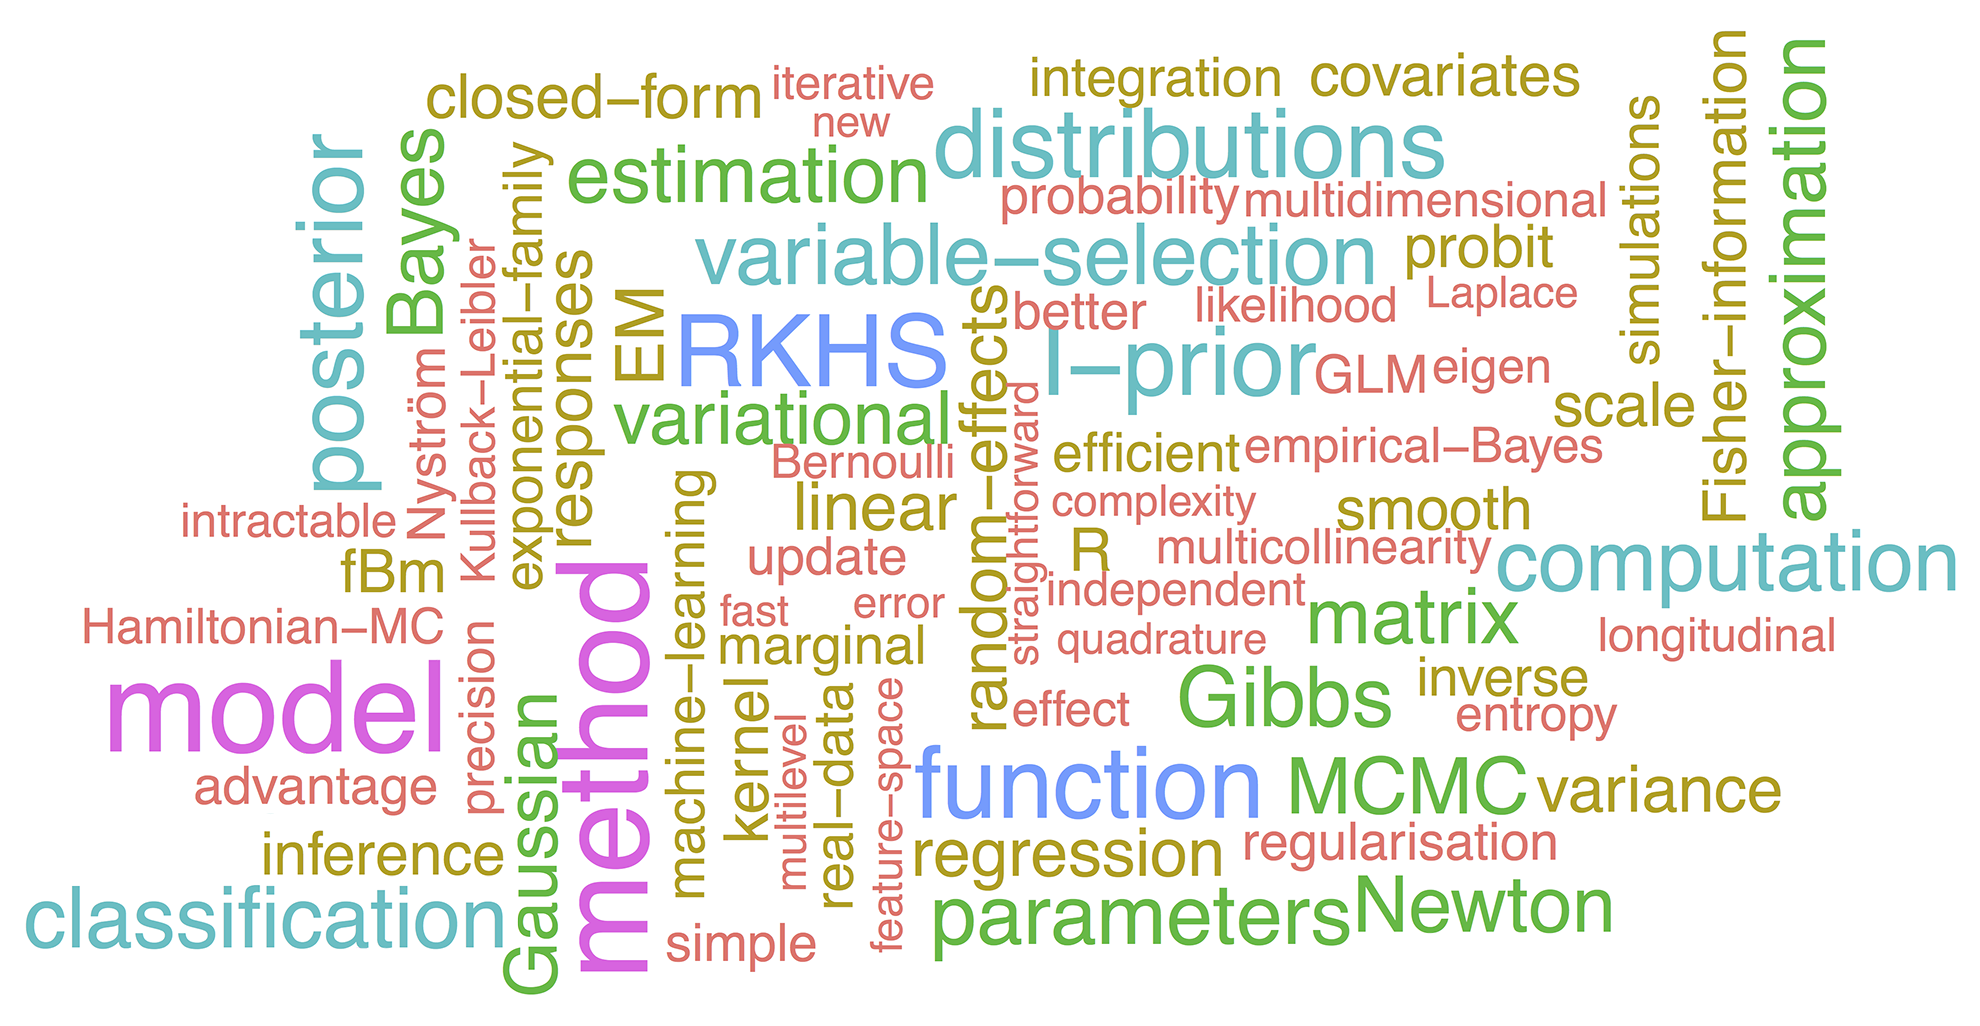
\includegraphics[width=\linewidth]{figure/keyword.png}
\end{figure}

% Introduction -----------------------------------------------------------------
\vspace{-12pt}
\begin{block}{Introduction}

Consider the following regression model for $i=1,\dots,n$:
~\\[-21pt]
\begin{align}\label{eq:normalmodel}
  \begin{gathered}
      y_i = \alpha + f(x_i) + \epsilon_i \\
    (\epsilon_1, \dots, \epsilon_n)^\top \sim \N_n(0,\Psi^{-1})
  \end{gathered}
\end{align}
~\\[-7pt]
where $y_i \in \bbR$, $x \in \cX$, and $f \in \cF$. Let $\cF$ be a reproducing kernel Hilbert space (RKHS) with kernel $h_\lambda:\cX \times \cX \to \bbR$. The Fisher information for $f$ evaluated at $x$ and $x'$ is
~\\[-22pt]
\begin{align}
  \cI\big(f(x), f(x')\big) = \sum_{k=1}^n \sum_{l=1}^n \Psi_{k,l} h_\lambda(x,x_k) h_\lambda(x',x_l).
\end{align}

\setbeamercolor{block alerted title}{fg=white,bg=colgrey} % Change the alert block title colors
\setbeamercolor{block alerted body}{fg=black,bg=white} % Change the alert block body colors
\begin{alertblock}{The I-prior}

The entropy maximising prior distribution for $f$, subject to identifying constraints, is 
~\\[-18pt]
\[
  \bff = \big(f(x_1),\dots,f(x_n) \big)^\top \sim \N_n \big(\bff_0, \cI[f] \big).
\]
~\\[-23pt]
Equivalently, $f(x) = f_0(x) + \sum_{i=1}^n h_\lambda(x,x_i)w_i$, with
~\\[-18pt]
\[
  (w_1, \dots, w_n)^\top \sim \N_n(0,\Psi).
\]
\vspace{-15pt}

\end{alertblock}

\vspace{-10pt}
Of interest are 

\newcommand{\new}{{\text{new}}}
\begin{itemize}
  \item the posterior distribution for the regression function
  \[
    p(\bff|\by) = \frac{p(\by|\bff) p(\bff)}{\int p(\by|\bff) p(\bff) \d \by}; \text{and}
  \]
  \item the posterior predictive distribution given new data
  \[
    p(y_\new|\by) = \int p(y_\new|f_\new,\by) p(f_\new|\by) \d f_\new.
  \]
\end{itemize}
\vspace{5pt}
Model parameters (error precision $\Psi$, RKHS scale parameters $\lambda$, and any others) may need to be estimated.
%, e.g. using likelihood methods or even MCMC.

\end{block}

% A Unifying Regression --------------------------------------------------------
\vspace{15pt}
\begin{block}{A Unified Regression Framework}

\begin{itemize}
%  \setlength\itemsep{0.3em}
  \item Multiple linear regression (linear RKHS)
%  \vspace{5pt}
%  \[
%    f(x_i) = \langle x_i,\beta \rangle
%  \]
%  \vspace{-35pt}
  \item Smoothing models (fBm RKHS)
  \item Multilevel regression (ANOVA RKHS: linear \& Pearson)
  \vspace{5pt}
  \[
      f(x_i^{(j)}) = f_1(j) + f_2(x_i^{(j)}) + f_{1:2}(x_i^{(j)}, j)
  \]
  \vspace{-35pt}  
  \item Longitudinal modelling (ANOVA RKHS: fBm \& Pearson)
  \vspace{-21pt}
  \[
    f(x_i, t_i) = f_1(t_i) + f_2(x_{i}) + f_{1:2}(x_{i},t_i)
  \]
  \vspace{-33pt}
  \item Functional covariates ($\cX$ is a Hilbert-Sobolev space)
\end{itemize}

\end{block}

\end{column}  % End of the first column

%%%%%%%%%%%%%%%%%%%%%%%%%%%%%%%%%%%%%%%%%%%%%%%%%%%%%%%%%%%%%%%%%%%%%%%%%%%%%%%%
%%% COLUMNS 2, 3, 4 %%%%%%%%%%%%%%%%%%%%%%%%%%%%%%%%%%%%%%%%%%%%%%%%%%%%%%%%%%%%
%%%%%%%%%%%%%%%%%%%%%%%%%%%%%%%%%%%%%%%%%%%%%%%%%%%%%%%%%%%%%%%%%%%%%%%%%%%%%%%%
\spacercolumn
\begin{column}{\threecolwid}
% figure spanning 2,3,4 is near the end
\vspace{-40pt}  

%%%%%%%%%%%%%%%%%%%%%%%%%%%%%%%%%%%%%%%%%%%%%%%%%%%%%%%%%%%%%%%%%%%%%%%%%%%%%%%%
%%% FIGURE SPANNING COLUMNS 2-3 %%%%%%%%%%%%%%%%%%%%%%%%%%%%%%%%%%%%%%%%%%%%%%%%
%%%%%%%%%%%%%%%%%%%%%%%%%%%%%%%%%%%%%%%%%%%%%%%%%%%%%%%%%%%%%%%%%%%%%%%%%%%%%%%%
\begin{columns}[t,totalwidth=\twocolwid]
\begin{column}{\twocolwid}  % columns that is two columns wide

% I-prior figures --------------------------------------------------------------
\vspace{-0.5cm}
\begin{figure}
\includegraphics[width=0.33\linewidth]{figure/kernel_path_canonical}
\includegraphics[width=0.33\linewidth]{figure/kernel_path_fbm}
\includegraphics[width=0.33\linewidth]{figure/kernel_path_pearson}
\vspace{-1.6cm}
\caption{(L-R) Sample paths from the linear, fractional Brownian motion (fBm), and Pearson RKHS. The (reproducing) kernels corresponding to each RKHS are: $h_\lambda(x,x') = \lambda  \langle x,x' \rangle_\cX$ (linear), $h_\lambda(x,x') = -\frac{\lambda}{2} \big( \norm{x-x'}_\cX^{2\gamma} - \norm{x}_\cX^{2\gamma} - \norm{x'}_\cX^{2\gamma}\big)$ (fBm), and $h_\lambda(x,x') = \lambda \big( {\delta_{xx'}} / {\Prob[X=x]} - 1 \big)$ (Pearson).}
\end{figure}

%%%%%%%%%%%%%%%%%%%%%%%%%%%%%%%%%%%%%%%%%%%%%%%%%%%%%%%%%%%%%%%%%%%%%%%%%%%%%%%%
%%% SECOND COLUMN %%%%%%%%%%%%%%%%%%%%%%%%%%%%%%%%%%%%%%%%%%%%%%%%%%%%%%%%%%%%%%
%%%%%%%%%%%%%%%%%%%%%%%%%%%%%%%%%%%%%%%%%%%%%%%%%%%%%%%%%%%%%%%%%%%%%%%%%%%%%%%%
\begin{columns}[t,totalwidth=\twocolwid]  % split the column
\begin{column}{\onecolwid}  % The first column within column 2 (column 2.1)

% Categorical responses --------------------------------------------------------
\vspace{5pt}
\begin{block}{Categorical Responses}
\vspace{2pt}

When each $y_i \in \{ 1,\dots,m \}$, normality assumptions are violated.
Model instead $y_i = \argmax_k y_{ik}^*\,$, where %for $j=1,\dots,m$,
~\\[-19pt]
\begin{align}\label{eq:iprobit}
  \begin{gathered}
    y_{ij}^* = \alpha_j + f_j(x_i) + \epsilon_{ij} \\    
%    \text{vec}\left( \epsilon_{ij} \right)_{i,j} \sim \N_{nm}\big(0, \Sigma \otimes \Psi^{-1}\big)
    (\epsilon_{i1},\dots,\epsilon_{im})^\top \sim \N_m(0, \Sigma) \\
  \end{gathered}
\end{align}
~\\[-5pt]
with $\Cov(\epsilon_{ij},\epsilon_{kj}) = 0$, for all $i\neq k$, $j=1,\dots,m$, and iid I-priors on $\bff_i = \big(f_1(x_i),\dots,f_m(x_i) \big)^\top$.
Class probabilities $p_{ij}$ are obtained using a \emph{truncated $m$-variate normal} density
~\\[-8pt]
\[
  p_{ij} = 
%  \int \ind\left[\{y_{ij}^* > y_{ik}^* | k \neq j \} \right] \cdot 
  \hspace{-1.3cm}
  \mathop{\int}_{\{y_{ij}^* > y_{ik}^* \,|\, k \neq j \}}
  \hspace{-1.3cm}
  \N_m(\by^*_i \,|\, \bff_i,\Sigma) \d\by_i^* \, =: \, g_j^{-1}(\bff_i).
\]
~\\[-10pt]
Now, the marginal, on which the posterior depends,
~\\[-16pt]
\[
  p(\by) = \int \prod_{i=1}^n \prod_{j=1}^m \left[ \Big\{ g_j^{-1}( \bff_i ) \Big\}^{[y_i = j]} \cdot \N_{m}(\bff_j \,|\, \bff_{0}, \cI[f]) \d \bff_j \right],
\]
~\\[-4pt]
cannot be found in closed form.
By working in a fully Bayesian setting, we append model parameters and employ a \emph{variational approximation}.
 
\end{block}

\end{column} % End of column 2.1

%%%%%%%%%%%%%%%%%%%%%%%%%%%%%%%%%%%%%%%%%%%%%%%%%%%%%%%%%%%%%%%%%%%%%%%%%%%%%%%%
%%% THIRD COLUMN %%%%%%%%%%%%%%%%%%%%%%%%%%%%%%%%%%%%%%%%%%%%%%%%%%%%%%%%%%%%%%%
%%%%%%%%%%%%%%%%%%%%%%%%%%%%%%%%%%%%%%%%%%%%%%%%%%%%%%%%%%%%%%%%%%%%%%%%%%%%%%%%
\begin{column}{\onecolwid}  % The second column within column 2 (column 2.2)

\vspace{5pt}
\begin{block}{Spatio-Temporal Modelling of BTB}
\vspace{2pt}

Determine the existence of spatial segregation of multiple types of bovine tuberculosis (BTB) in Cornwall, and whether the spatial distribution had changed over time.

\begin{itemize}
  \item Constant model (constant RKHS)
  \vspace{4pt}
  \[
    p_{ij} = g^{-1}_j\big( \alpha_k \big)_{k=1}^m
  \]
  \vspace{-32pt}
  \item Spatial segregation (fBm RKHS)
  \vspace{3pt}
  \[
    p_{ij} = g^{-1}_j\big(\alpha_k + f_{1k}(x_i) \big)_{k=1}^m
  \]
  \vspace{-34pt}  
  \item Spatio-temporal segregation (ANOVA RKHS)
  \vspace{6pt}
  \[
    p_{ij} = g^{-1}_j\big(\alpha_k + f_{1k}(x_i) + f_{2k}(t_i) + f_{12k}(x_i,t_i) \big)_{k=1}^m
  \]
  \vspace{-38pt}
\end{itemize}  

Evidence Lower Bound (ELBO) values for the three models are -1197.4, -665.3, and -656.2 respectively.
% -656.2  spatio-temporal
% -664.7  spatio-period
\end{block}

\vspace{2pt}
\begin{block}{Detecting Cardiac Arrhythmia}
\vspace{2pt}
  
Predict whether patients suffers from a cardiac disease based on features such as age, height, weight and a myriad of electrocardiogram (ECG) data ($p=271$).  
  
\end{block}

\end{column}

\end{columns}

\end{column}



%%%%%%%%%%%%%%%%%%%%%%%%%%%%%%%%%%%%%%%%%%%%%%%%%%%%%%%%%%%%%%%%%%%%%%%%%%%%%%%%
%%% FOURTH COLUMN %%%%%%%%%%%%%%%%%%%%%%%%%%%%%%%%%%%%%%%%%%%%%%%%%%%%%%%%%%%%%%
%%%%%%%%%%%%%%%%%%%%%%%%%%%%%%%%%%%%%%%%%%%%%%%%%%%%%%%%%%%%%%%%%%%%%%%%%%%%%%%%
\spacercolumn
\begin{column}{\onecolwid}



% Detecting Cardiac Arrhythmia -------------------------------------------------
\vspace{-30pt}

\begin{table}
  \caption{Mean out-of-sample misclassification rates and standard errors for 100 runs of various training ($n$) and test ($451-n$) sizes for the cardiac arrhythmia binary classification task.}
  \vspace{10pt}
  \begin{tabular}{l r r r}
  \toprule
  &\multicolumn{3}{ c }{\textbf{Misclassification rate (\%)}} \\
  \textbf{Method\hspace{15.5mm}}
  & \hspace{0.5cm} \textbf{\hspace{14mm}\boldmath$n = 50$} 
  & \hspace{0.5cm} \textbf{\hspace{10.5mm}\boldmath$n = 100$} 
  & \hspace{0.5cm} \textbf{\hspace{10.5mm}\boldmath$n = 200$} \\
  \midrule
  {I-probit (linear)}  & 34.5 (0.4) & 31.4 (0.4) & 29.7 (0.4) \\
  {I-probit (fBm)}     & 34.7 (0.6) & 27.3 (0.3) & 24.5 (0.3) \\[0.5em]
  {GP (Gaussian)}      & 37.3 (0.4) & 33.8 (0.4) & 29.3 (0.4) \\  
  {L-1 logistic}       & 34.9 (0.4) & 30.5 (0.3) & 26.1 (0.3) \\[0.5em] 
  {SVM (linear)}       & 36.2 (0.5) & 35.6 (0.4) & 35.2 (0.4) \\
  {SVM (Gaussian)}     & 48.4 (0.5) & 47.2 (0.5) & 46.9 (0.4) \\[0.5em] 
  {RF}                 & 31.7 (0.4) & 26.7 (0.3) & 22.4 (0.3) \\
  {$k$-NN}             & 40.6 (0.3) & 38.9 (0.3) & 35.8 (0.4) \\
  \bottomrule
  \end{tabular}
\end{table}  
\vspace{13pt}
%  {I-probit (linear)}  & 34.5 (0.43) & 31.4 (0.38) & 29.7 (0.35) \\
%  {I-probit (fBm)}     & 34.7 (0.59) & 27.3 (0.29) & 24.5 (0.30) \\[0.5em]
%  {GP (Gaussian)}      & 37.3 (0.42) & 33.8 (0.40) & 29.3 (0.35) \\  
%  {L-1 logistic}       & 34.9 (0.42) & 30.5 (0.34) & 26.1 (0.27) \\[0.5em] 
%  {SVM}                & 36.2 (0.47) & 35.6 (0.39) & 35.2 (0.35) \\
%  {RF}                 & 31.7 (0.39) & 26.7 (0.29) & 22.4 (0.31) \\[0.5em] 
%  {$k$-NN}             & 40.6 (0.33) & 38.9 (0.33) & 35.8 (0.36) \\

% Conclusion -------------------------------------------------------------------
\setbeamercolor{block alerted title}{fg=white,bg=colgrey} % Change the alert block title colors
\setbeamercolor{block alerted body}{fg=black,bg=white} % Change the alert block body colors
\begin{alertblock}{Conclusions}

\begin{itemize}
%  \item The EM algorithm provides a straightforward and efficient method of estimating I-prior models.
  \item Simple estimation of various categorical models:
  \begin{itemize}
    \item Choice models (with or without IIA);
    \item Random-effects models;
    \item Binary and multiclass classification.
  \end{itemize}
  \item Inference is straightforward (e.g. model compari- son or transformed parameter significance).
  \item Often gives better predictions.
\end{itemize}

\end{alertblock}



% References -------------------------------------------------------------------
\vspace{-1mm}
\begin{block}{References}

\vspace{-19pt}
\nocite{*}
\bibliographystyle{unsrt}
\small{\bibliography{bib/phd-poster}}

\end{block}

\end{column}
 

 
\end{columns}

\vspace{-18pt}
\begin{figure}
  \includegraphics[width=0.246\linewidth]{figure/btb_spat_1}
  \includegraphics[width=0.246\linewidth]{figure/btb_spat_2}
  \includegraphics[width=0.246\linewidth]{figure/btb_spat_3}
  \includegraphics[width=0.246\linewidth]{figure/btb_spat_4}
  \vspace{-0.7cm}
  \caption{Predicted probability surfaces for BTB contraction in Cornwall for the four largest spoligotypes of the bacterium \emph{Mycobacterium bovis} over the entire time period 1989--2002.}
\end{figure}



\end{column}  % End of 3-span column




%%%%%%%%%%%%%%%%%%%%%%%%%%%%%%%%%%%%%%%%%%%%%%%%%%%%%%%%%%%%%%%%%%%%%%%%%%%%%%%%
%%% END DOCUMENT %%%%%%%%%%%%%%%%%%%%%%%%%%%%%%%%%%%%%%%%%%%%%%%%%%%%%%%%%%%%%%%
%%%%%%%%%%%%%%%%%%%%%%%%%%%%%%%%%%%%%%%%%%%%%%%%%%%%%%%%%%%%%%%%%%%%%%%%%%%%%%%%
\spacercolumn
\end{columns} % End of all the columns in the poster
\end{frame} % End of the enclosing frame
\end{document}
